\documentclass[journal,12pt,twocolumn]{IEEEtran}
\usepackage{setspace}
\usepackage{gensymb}
\singlespacing
\usepackage[cmex10]{amsmath}
\usepackage{amsthm}
\usepackage{mathrsfs}
\usepackage{txfonts}
\usepackage{stfloats}
\usepackage{bm}
\usepackage{cite}
\usepackage{cases}
\usepackage{subfig}
\usepackage{longtable}
\usepackage{multirow}
\usepackage{enumitem}
\usepackage{mathtools}
\usepackage{tikz}
\usepackage{circuitikz}
\usepackage{verbatim}
\usepackage[breaklinks=true]{hyperref}
\usepackage{tkz-euclide} % loads  TikZ and tkz-base
\usepackage{listings}
\usepackage{color}    
\usepackage{array}    
\usepackage{longtable}
\usepackage{calc}     
\usepackage{multirow} 
\usepackage{hhline}   
\usepackage{ifthen}   
\usepackage{lscape}     
\usepackage{chngcntr}
\DeclareMathOperator*{\Res}{Res}
\renewcommand\thesection{\arabic{section}}
\renewcommand\thesubsection{\thesection.\arabic{subsection}}
\renewcommand\thesubsubsection{\thesubsection.\arabic{subsubsection}}

\renewcommand\thesectiondis{\arabic{section}}
\renewcommand\thesubsectiondis{\thesectiondis.\arabic{subsection}}
\renewcommand\thesubsubsectiondis{\thesubsectiondis.\arabic{subsubsection}}
\renewcommand\thetable{\arabic{table}}
% correct bad hyphenation here
\hyphenation{op-tical net-works semi-conduc-tor}
\def\inputGnumericTable{}                                 %%

\lstset{
%language=C,
frame=single, 
breaklines=true,
columns=fullflexible,
literate=
{-}{$\rightarrow{}$}{1},
}
%\lstset{
%language=tex,
%frame=single, 
%breaklines=true
%}

\DeclareMathOperator*{\argmax}{arg\,max}
\DeclareMathOperator*{\argmin}{arg\,min}
\begin{document}
\newtheorem{theorem}{Theorem}[section]
\newtheorem{problem}{Problem}
\newtheorem{proposition}{Proposition}[section]
\newtheorem{lemma}{Lemma}[section]
\newtheorem{corollary}[theorem]{Corollary}
\newtheorem{example}{Example}[section]
\newtheorem{definition}[problem]{Definition}
\newcommand{\BEQA}{\begin{eqnarray}}
\newcommand{\EEQA}{\end{eqnarray}}
\newcommand{\define}{\stackrel{\triangle}{=}}
\bibliographystyle{IEEEtran}
\providecommand{\mbf}{\mathbf}
\providecommand{\pr}[1]{\ensuremath{\Pr\left(#1\right)}}
\providecommand{\qfunc}[1]{\ensuremath{Q\left(#1\right)}}
\providecommand{\sbrak}[1]{\ensuremath{{}\left[#1\right]}}
\providecommand{\lsbrak}[1]{\ensuremath{{}\left[#1\right.}}
\providecommand{\rsbrak}[1]{\ensuremath{{}\left.#1\right]}}
\providecommand{\brak}[1]{\ensuremath{\left(#1\right)}}
\providecommand{\lbrak}[1]{\ensuremath{\left(#1\right.}}
\providecommand{\rbrak}[1]{\ensuremath{\left.#1\right)}}
\providecommand{\cbrak}[1]{\ensuremath{\left\{#1\right\}}}
\providecommand{\lcbrak}[1]{\ensuremath{\left\{#1\right.}}
\providecommand{\rcbrak}[1]{\ensuremath{\left.#1\right\}}}
\theoremstyle{remark}
\newtheorem{rem}{Remark}
\newcommand{\sgn}{\mathop{\mathrm{sgn}}}
\newcommand{\re}{\mathop{\mathrm{Re}}}
\providecommand{\abs}[1]{\left\vert#1\right\vert}
\providecommand{\res}[1]{\Res\displaylimits_{#1}} 
\providecommand{\norm}[1]{\left\lVert#1\right\rVert}
\providecommand{\mtx}[1]{\mathbf{#1}}
\providecommand{\mean}[1]{E\left[ #1 \right]}   
\providecommand{\fourier}{\overset{\mathcal{F}}{ \rightleftharpoons}}
\providecommand{\system}[1]{\overset{\mathcal{#1}}{ \longleftrightarrow}}
\newcommand{\solution}{\noindent \textbf{Solution: }}
\newcommand{\cosec}{\,\text{cosec}\,}
\providecommand{\dec}[2]{\ensuremath{\overset{#1}{\underset{#2}{\gtrless}}}}
\newcommand{\myvec}[1]{\ensuremath{\begin{pmatrix}#1\end{pmatrix}}}
\newcommand{\mydet}[1]{\ensuremath{\begin{vmatrix}#1\end{vmatrix}}}
\renewcommand{\vec}[1]{\boldsymbol{\mathbf{#1}}}
\def\putbox#1#2#3{\makebox[0in][l]{\makebox[#1][l]{}\raisebox{\baselineskip}[0in][0in]{\raisebox{#2}[0in][0in]{#3}}}}
     \def\rightbox#1{\makebox[0in][r]{#1}}
     \def\centbox#1{\makebox[0in]{#1}}
     \def\topbox#1{\raisebox{-\baselineskip}[0in][0in]{#1}}
     \def\midbox#1{\raisebox{-0.5\baselineskip}[0in][0in]{#1}}

\vspace{3cm}
\title{Advanced DSP (EE5900)\\Homework Assignment 1}
\author{Gautam Singh\\CS21BTECH11018}
\maketitle
\bigskip

The transfer function in the \(s\)-domain is
\begin{align}
    \frac{Y\brak{s}}{X\brak{s}} = H\brak{s} = \frac{\frac{R}{L}s}{s^2 + \frac{R}{L}s + \frac{1}{LC}}.
    \label{eq:s-trans-func}
\end{align}

\begin{enumerate}[label=\theenumi.]
    \item To find the zeros, we set
    \begin{equation}
        Y\brak{s} = \frac{R}{L}s = 0 \implies s = 0.
    \end{equation}
    Thus, the only zero is
    \begin{equation}
        z_1 = 0. \label{eq:zeros}
    \end{equation}
    To find the poles, we set
    \begin{align}
        &X\brak{s} = s^2 + \frac{R}{L}s + \frac{1}{LC} = 0 \\
        &\brak{s + \frac{R}{2L}}^2 - \brak{\frac{R^2}{4L^2} - \frac{1}{LC}} = 0 \\
        &s = -\frac{R}{2L} \pm \sqrt{\frac{R^2}{4L^2} - \frac{1}{LC}}.
    \end{align}
    Thus, the poles of the system are 
    \begin{equation}
        p_1, p_2 = -\frac{R}{2L} \pm \sqrt{\frac{R^2}{4L^2} - \frac{1}{LC}}.
        \label{eq:poles}
    \end{equation}
    For various cases, the pole-zero plots are shown in 
    \autoref{fig:pole-zero-underdamping}, \autoref{fig:pole-zero-crit}, and
    \autoref{fig:pole-zero-overdamping}.
    \begin{figure}[!ht]
        \centering
        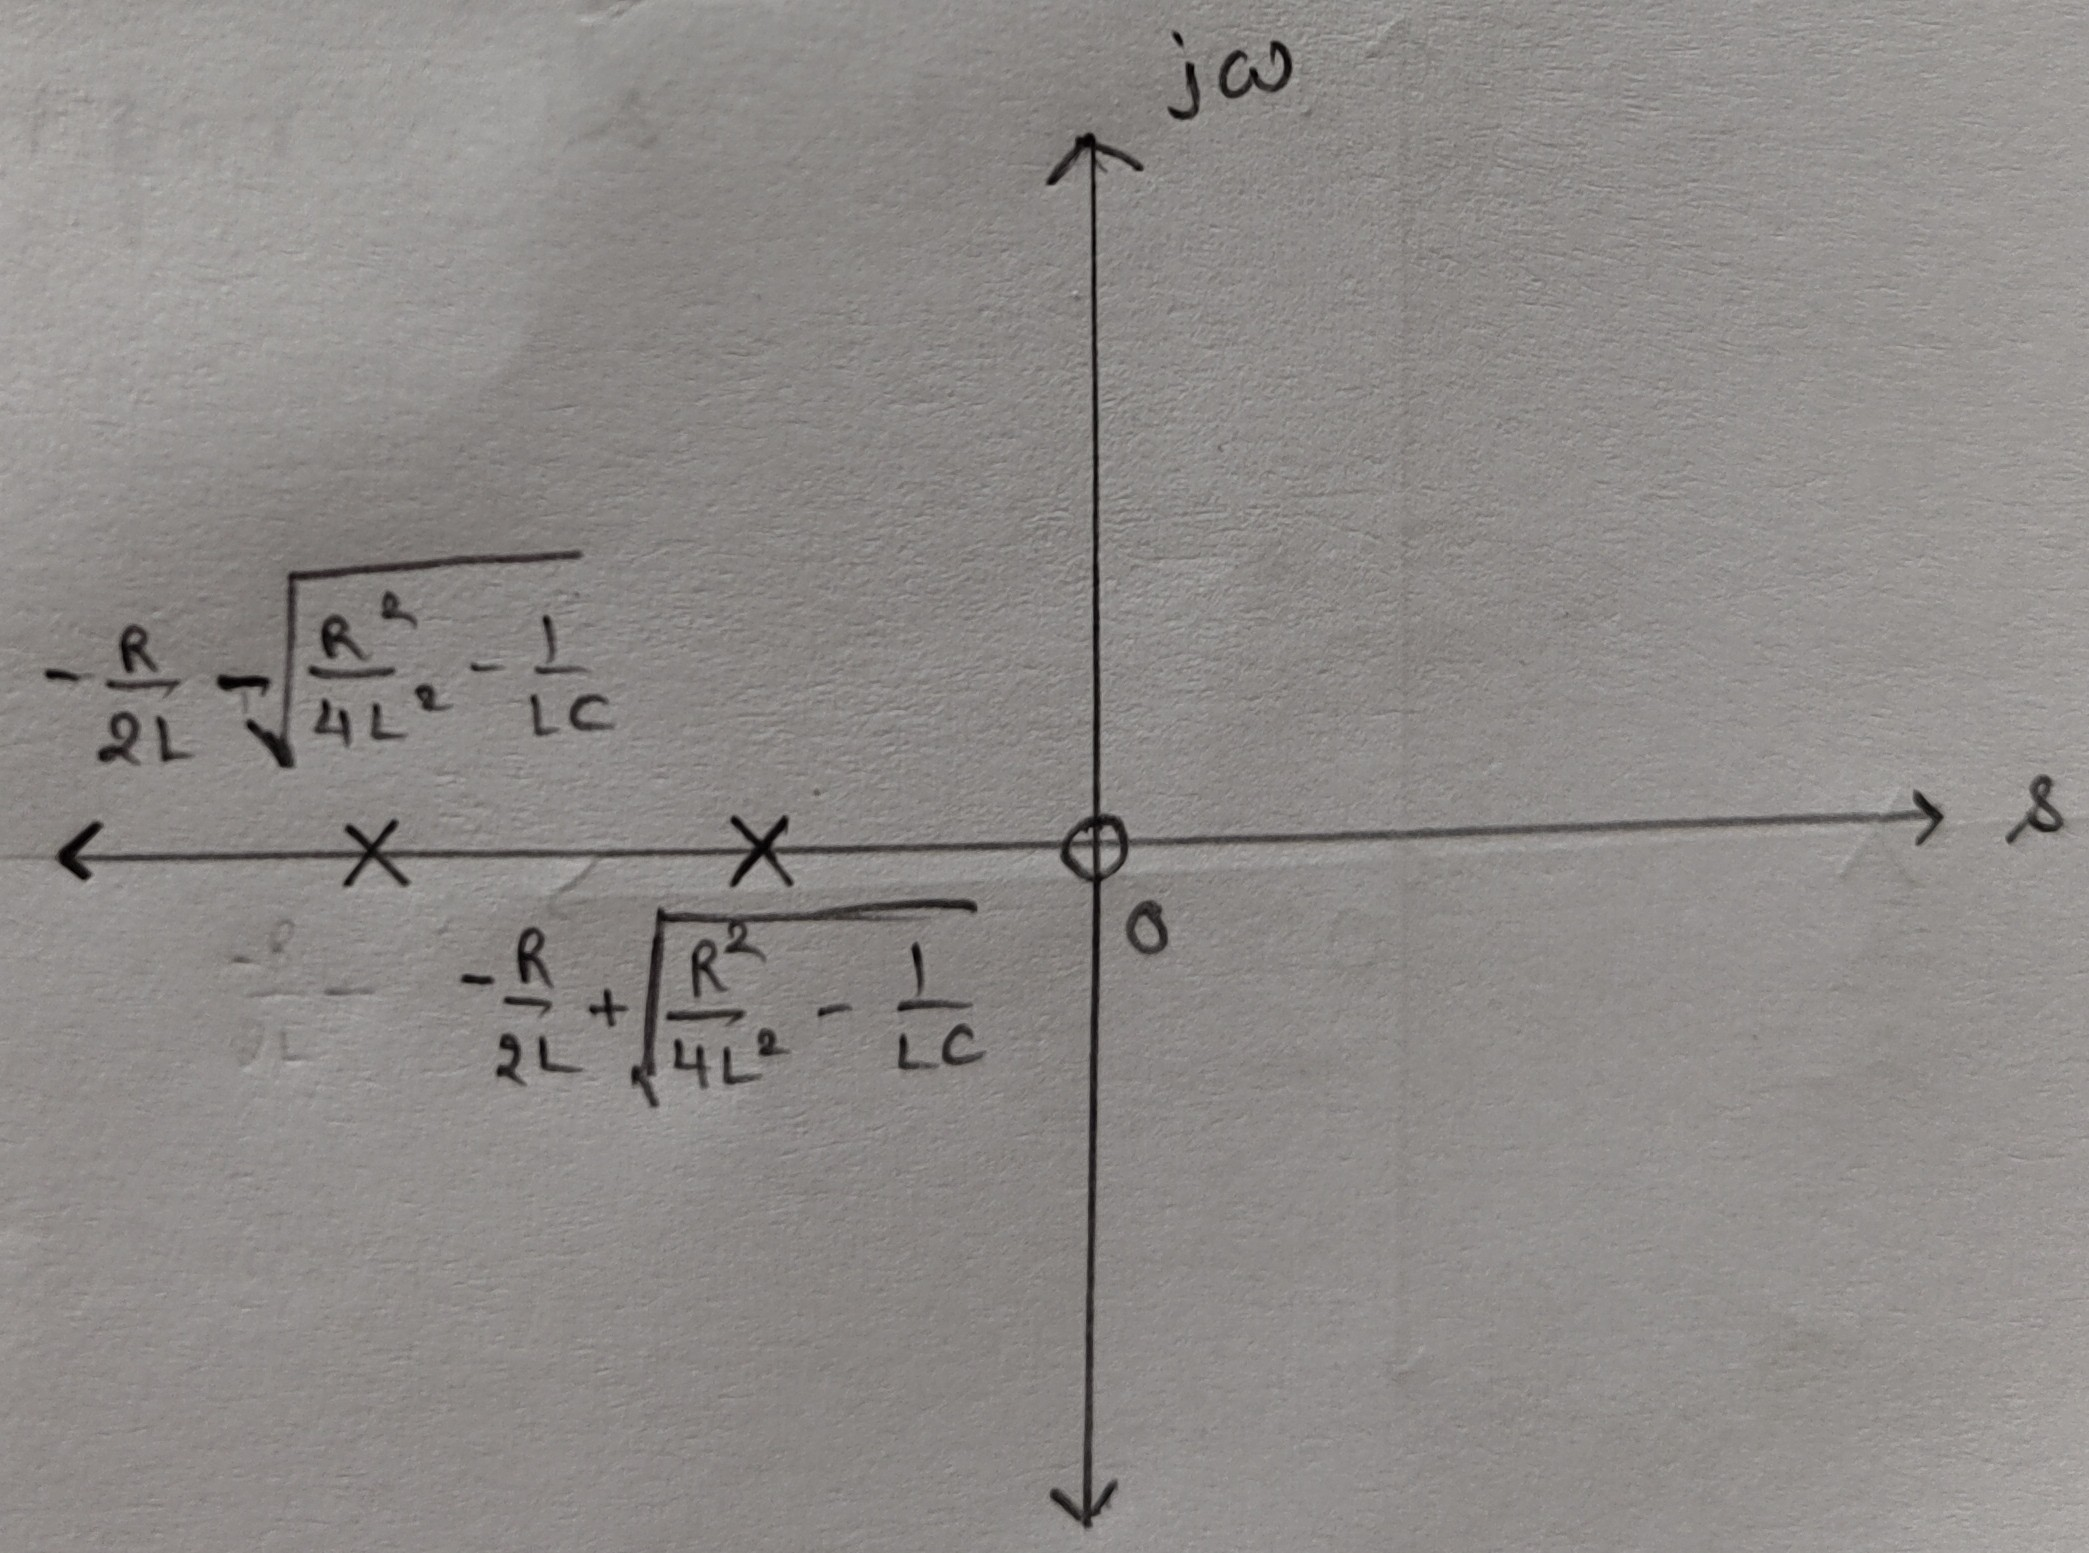
\includegraphics[width=\columnwidth]{figs/pole-zero-overdamping.jpg}
        \caption{Pole-zero plot when \(\frac{R^2}{4L^2} > \frac{1}{LC}\).}
        \label{fig:pole-zero-overdamping}
    \end{figure}
    \begin{figure}[!ht]
        \centering
        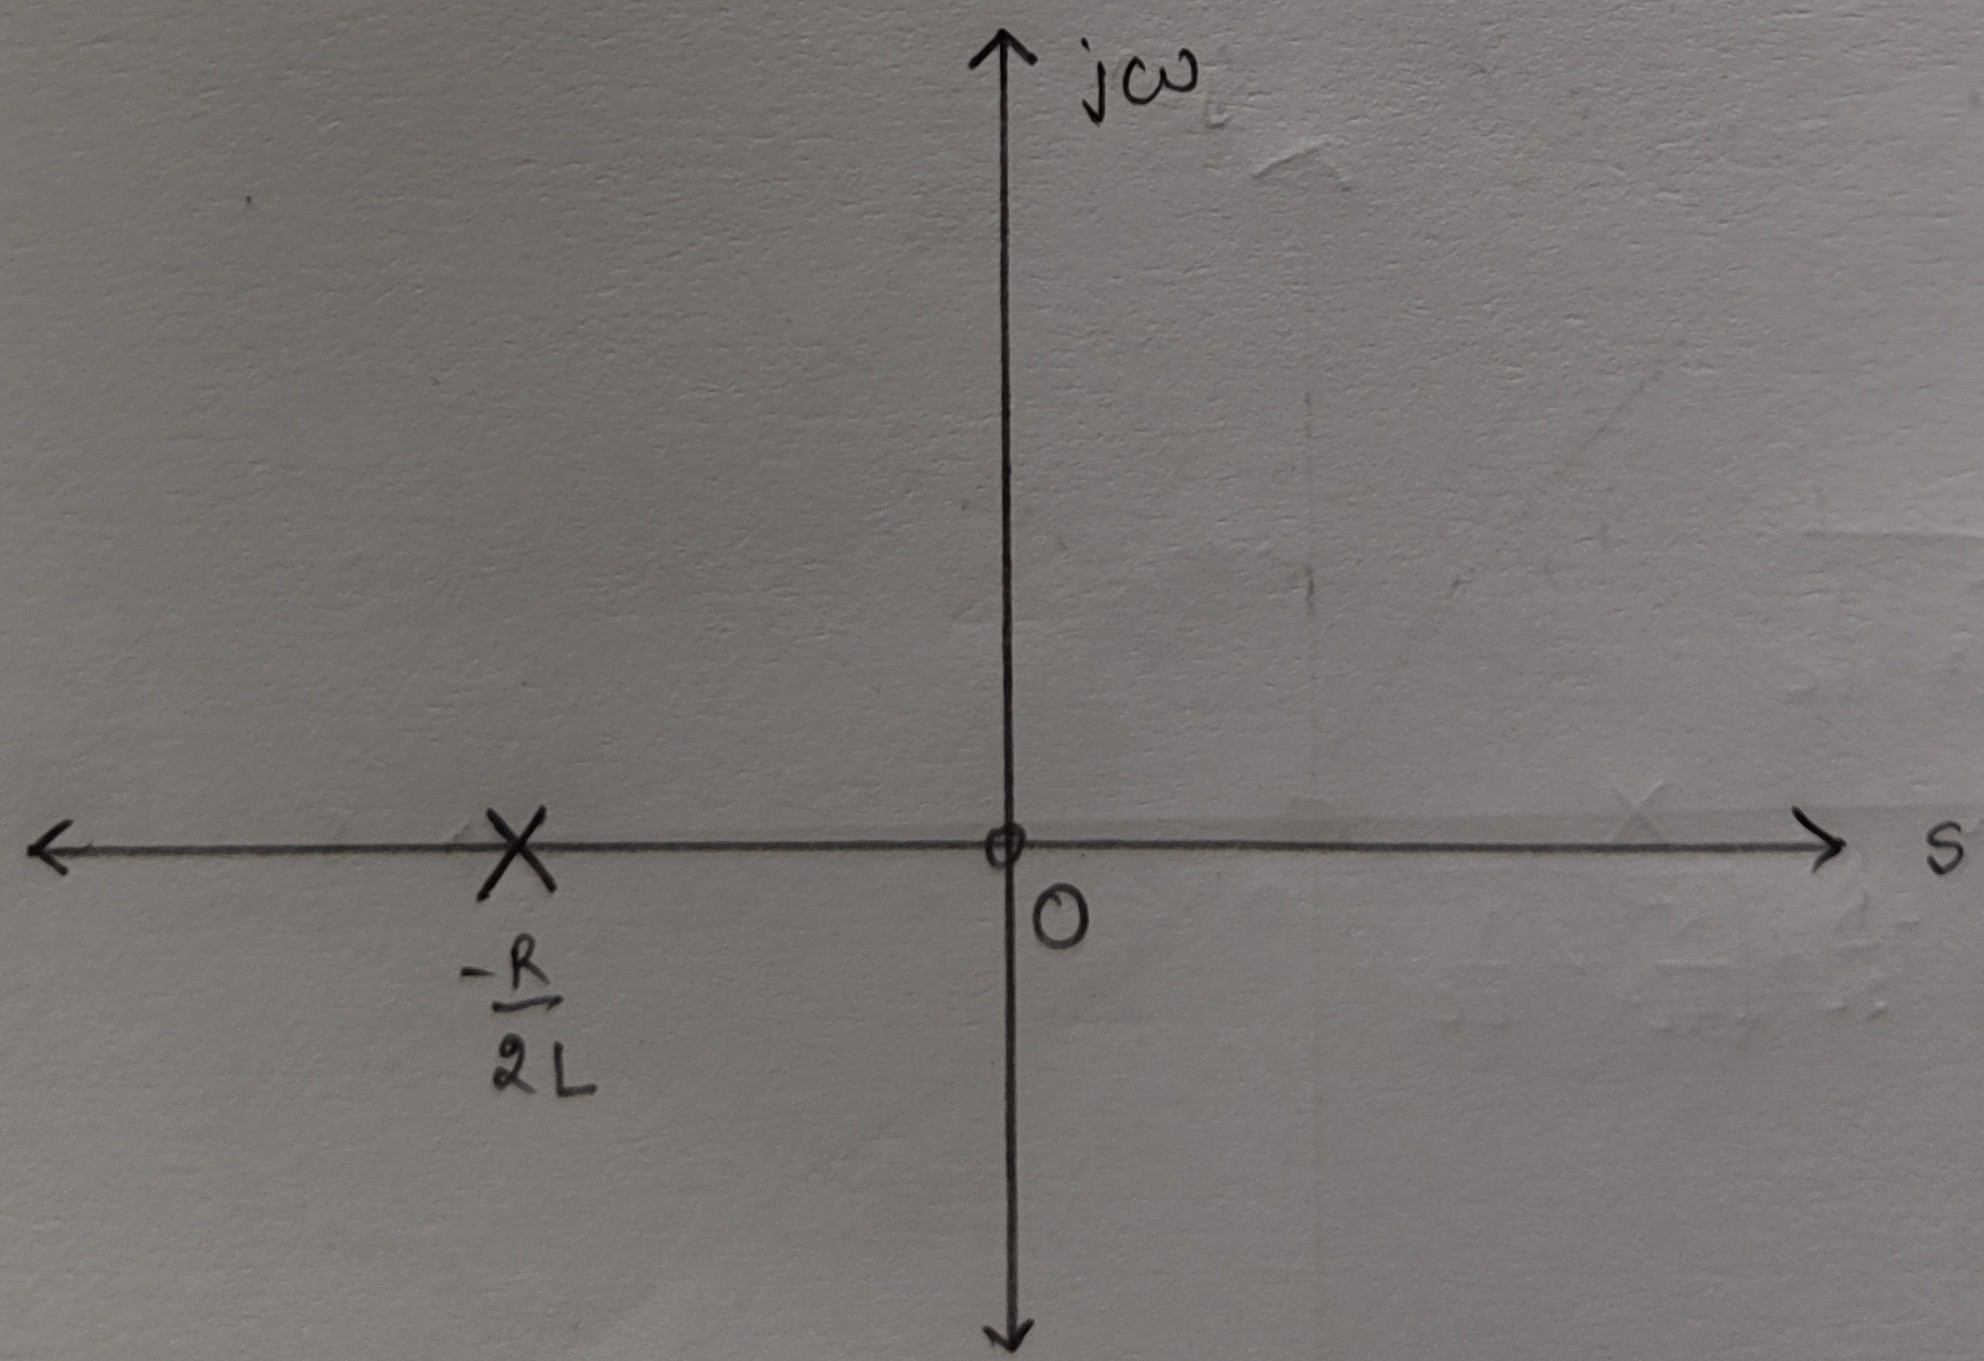
\includegraphics[width=\columnwidth]{figs/pole-zero-crit.jpg}
        \caption{Pole-zero plot when \(\frac{R^2}{4L^2} = \frac{1}{LC}\). The
        two poles are repeated.}
        \label{fig:pole-zero-crit}
    \end{figure}
    \begin{figure}[!ht]
        \centering
        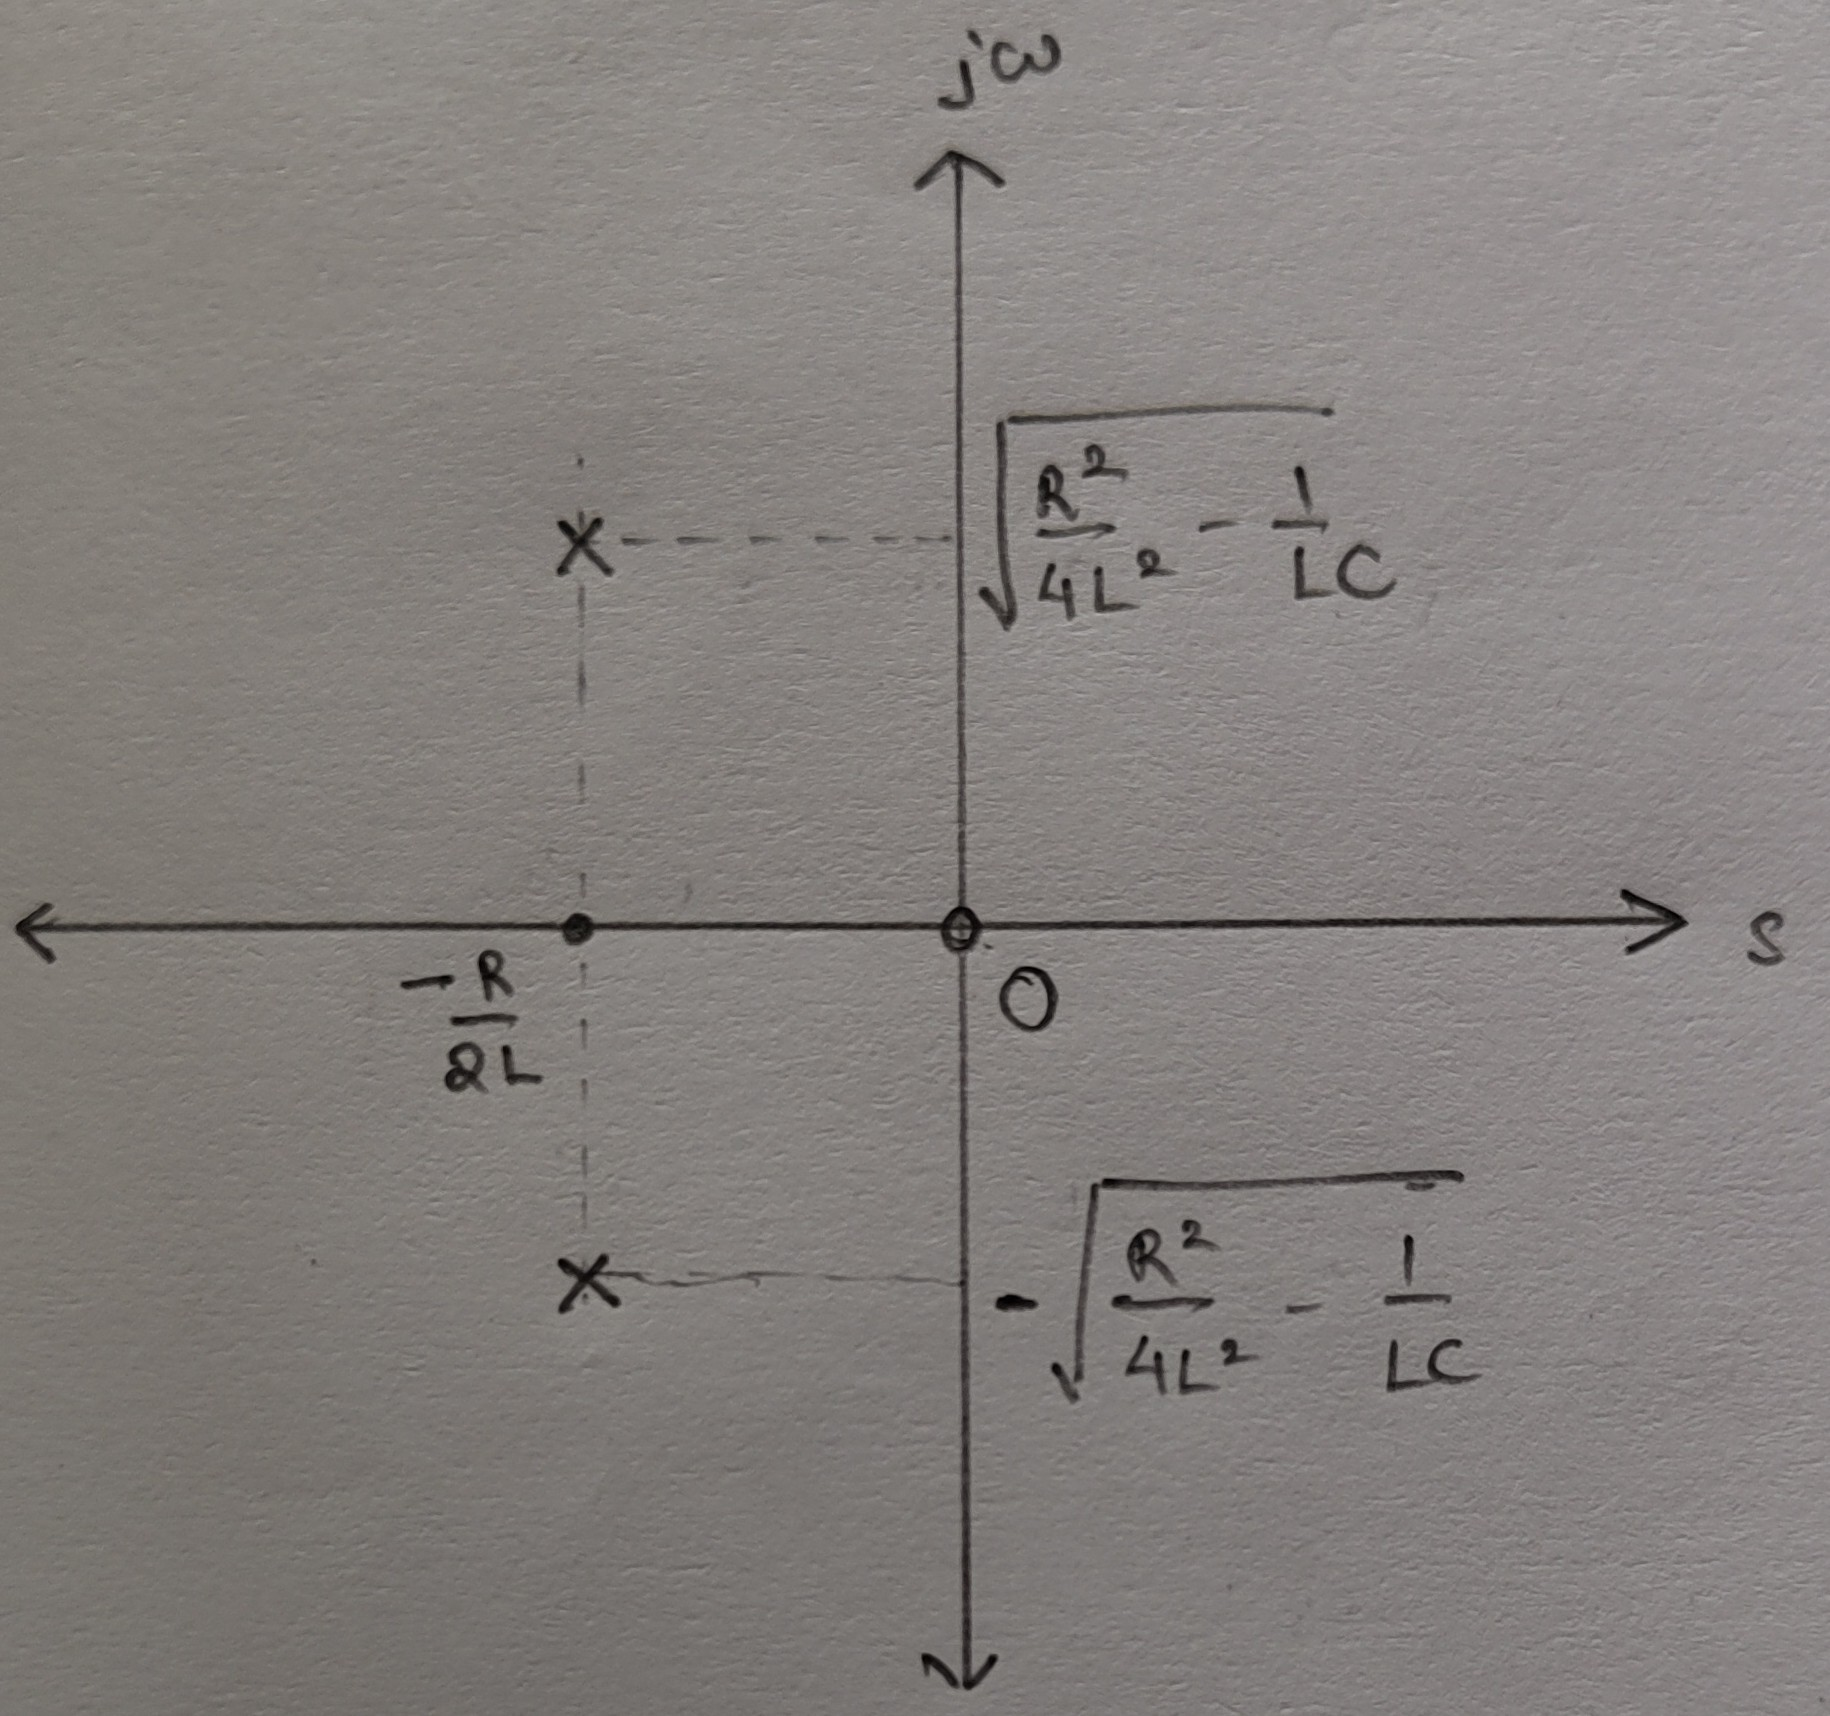
\includegraphics[width=\columnwidth]{figs/pole-zero-underdamping.jpg}
        \caption{Pole-zero plot when \(\frac{R^2}{4L^2} < \frac{1}{LC}\).}
        \label{fig:pole-zero-underdamping}
    \end{figure}
    Notice that \(H\brak{s}\) is rational and has conjugate poles, thus it will have
    a real-valued impulse response. The system is causal if we consider the
    region of convergence (ROC) which is to the right of all the poles, that is,
    \begin{equation}
        \re\brak{s} > \max\brak{\re\brak{p_1},\ \re\brak{p_2}}.
        \label{eq:causal-roc}
    \end{equation}
    From \eqref{eq:poles}, it is clear that
    \begin{equation}
        \re\brak{p_1} \ge \re\brak{p_2}.
    \end{equation}
    Now, for the system to be stable, we must consider the ROC which contains
    the imaginary axis in the \(s\)-domain. However,
    \begin{equation}
        \re\brak{p_1} \le -\frac{R}{2L} + \sqrt{\frac{R^2}{4L^2}-\frac{1}{LC}} < 0.
        \label{eq:real-p1}
    \end{equation}
    with equality iff \(\frac{R^2}{4L^2} \ge \frac{1}{LC}\). Therefore, the
    required condition on \(s\) is
    \begin{equation}
        \re\brak{s} > \re\brak{-\frac{R}{2L} + \sqrt{\frac{R^2}{4L^2} - \frac{1}{LC}}}.
        \label{eq:condition-s}
    \end{equation}

    \item Rewriting \eqref{eq:s-trans-func}, we have
    \begin{equation}
        \brak{sL+1+\frac{1}{sC}}\frac{Y\brak{s}}{R} = X\brak{s}.
        \label{eq:s-ckt}
    \end{equation}
    Taking the inverse Laplace transform on both sides of \eqref{eq:s-ckt},
    and using the identities for the Laplace pair \(f\brak{t},\ F\brak{s}\),
    \begin{align}
        f^{'}\brak{t} &\system{L} sF\brak{s} - f\brak{0}, \label{eq:laplace-diff} \\
        \int_{0}^tf\brak{t}dt &\system{L} \frac{F\brak{s}}{s}, \label{eq:laplace-int}
    \end{align}
    the required differential equation is
    \begin{equation}
        \frac{1}{R}\brak{L\frac{dy}{dt} + y\brak{t} + \frac{1}{C}\int_{0}^ty\brak{t}dt} = x\brak{t}.
        \label{eq:diff-rlc-s}
    \end{equation}

    \item Defining
    \begin{align}
        i\brak{t} &\define \frac{y\brak{t}}{R}, \label{eq:current-def} \\
        v\brak{t} &\define x\brak{t},
    \end{align}
    \eqref{eq:diff-rlc-s} becomes
    \begin{equation}
        L\frac{di}{dt} + Ri\brak{t} + \frac{1}{C}\int_{0}^ti\brak{t}dt = v\brak{t}.
        \label{eq:diff-rlc-t}
    \end{equation}
    This clearly represents a series RLC circuit with input voltage \(v\brak{t}\)
    and output voltage taken across \(R\), as shown in \autoref{fig:rlc}.
    \begin{figure}[!ht]
        \centering
        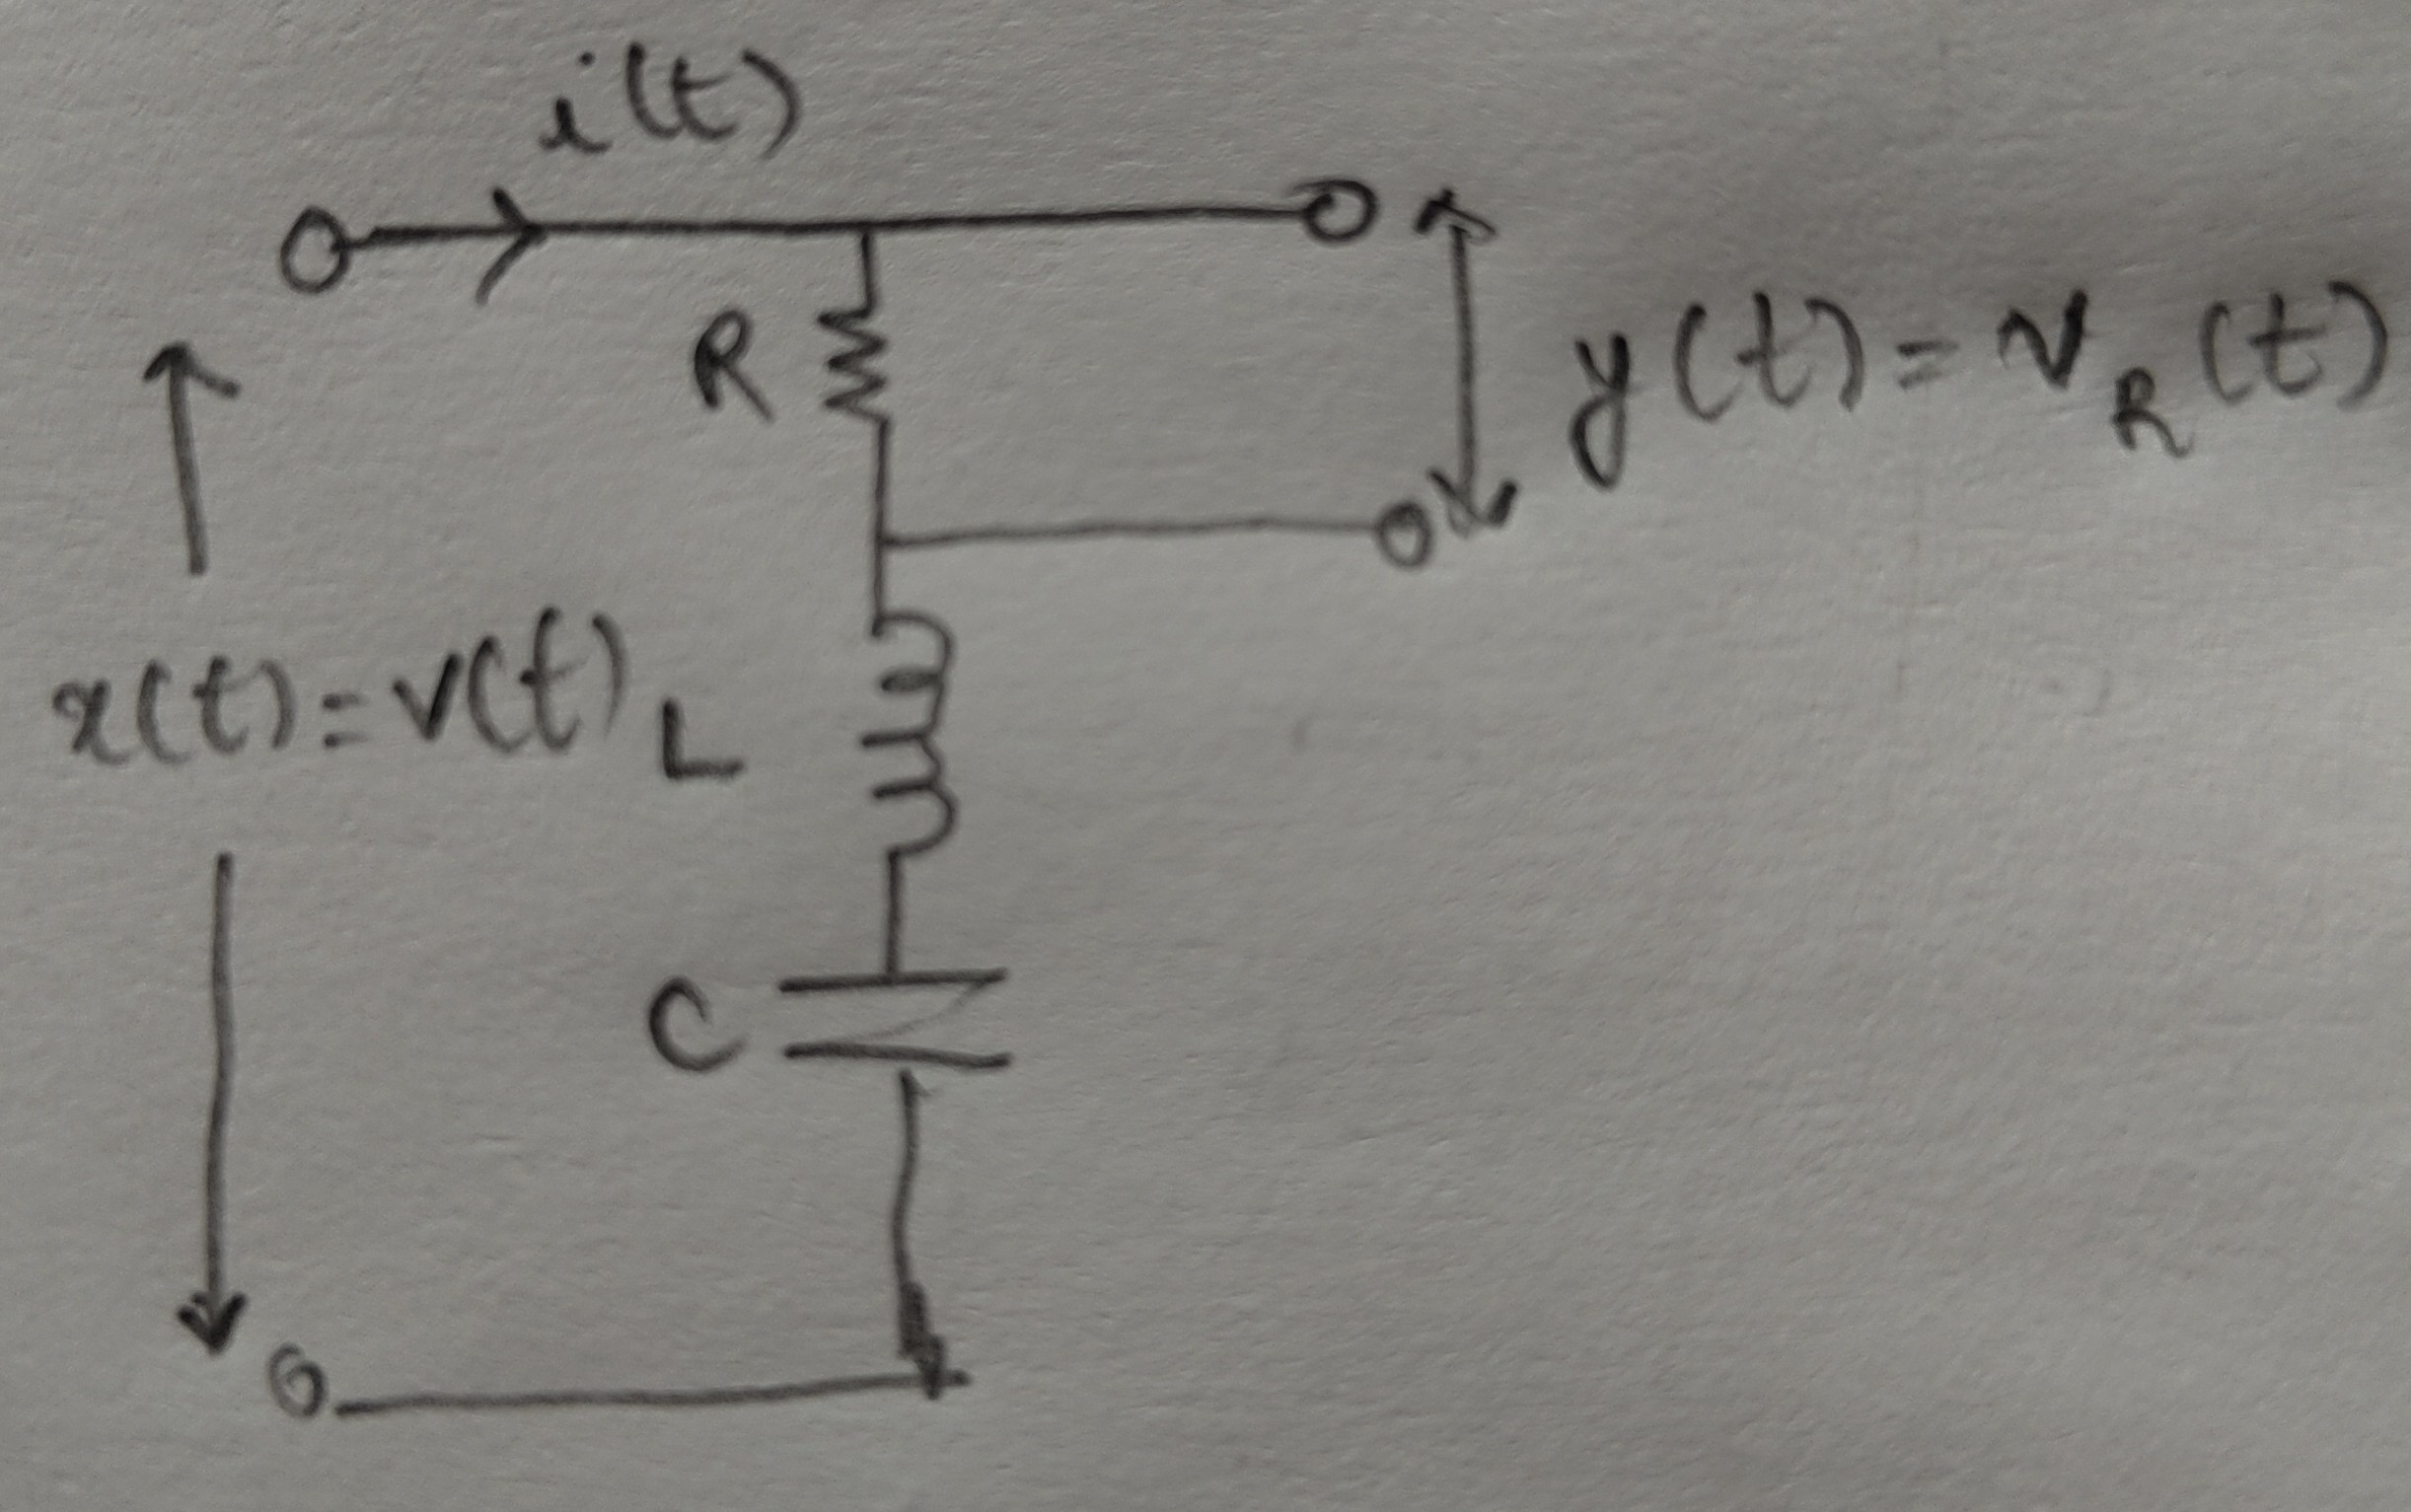
\includegraphics[width=\columnwidth]{figs/rlc.jpg}
        \caption{Series RLC circuit depicting \(x\brak{t}\) and \(y\brak{t}\).}
        \label{fig:rlc}
    \end{figure}

    \item From \eqref{eq:s-trans-func}, completing the square,
    \begin{equation}
        H\brak{s} = \frac{\frac{R}{L}s}{\brak{s + \frac{R}{2L}}^2 + \brak{\frac{1}{LC} - \frac{R^2}{4L^2}}}.
        \label{eq:s-trans-square}
    \end{equation}
    We define
    \begin{align}
        \alpha &\define \frac{R}{2L}, \label{eq:alpha-def} \\
        \omega_0 &\define \frac{1}{\sqrt{LC}}, \label{eq:omega-0-def} \\
    \end{align}
    where \(\alpha\) and \(\omega_0\) are the damping coefficient and resonance
    frequency respectively. Thus, we rewrite \eqref{eq:s-trans-square} as
    \begin{equation}
        H\brak{s} = \frac{2\alpha{}s}{\brak{s + \alpha}^2 + \brak{\omega_0^2-\alpha^2}}.
        \label{eq:s-trans-simplified}
    \end{equation}
    We have three cases.
    \begin{enumerate}
        \item \(\alpha < \omega_0\). This is called \emph{underdamping}.
        Defining
        \begin{equation}
            \omega \define \sqrt{\omega_0^2-\alpha^2}, \label{eq:omega-def}
        \end{equation}
        from \eqref{eq:s-trans-simplified},
        \begin{align}
            H\brak{s} &= \frac{2\alpha{}s}{\brak{s+\alpha}^2 + \omega^2} \label{eq:H-s-underdamping} \\ 
            &= \frac{2\alpha\brak{s + \alpha}}{\brak{s + \alpha}^2 + \omega^2} - \frac{2\alpha^2}{\omega^2}\frac{\omega^2}{\brak{s+\alpha}^2 + \omega^2}.
            \label{eq:s-trans-underdamping}
        \end{align}
        Taking the inverse Laplace Transform on both sides of
        \eqref{eq:s-trans-underdamping},
        \begin{equation}
            h\brak{t} = 2\alpha{}e^{-\alpha{}t}u\brak{t}\brak{\cos{\omega{}t} - \frac{\alpha}{\omega^2}\sin{\omega{}t}}.
            \label{eq:h-t-underdamping}
        \end{equation}

        \item \(\alpha = \omega_0\). This is called \emph{critical damping}.
        Here, \eqref{eq:s-trans-simplified} becomes
        \begin{align}
            H\brak{s} &= \frac{2\alpha{}s}{\brak{s+\alpha}^2} \label{eq:H-s-crit} \\
                      &= \frac{2\alpha}{\brak{s+\alpha}} - \frac{2\alpha^2}{\brak{s+\alpha}^2}.
            \label{eq:s-trans-crit}
        \end{align}
        Taking the inverse Laplace transform on both sides of
        \eqref{eq:s-trans-crit},
        \begin{equation}
            h\brak{t} = 2\alpha{}e^{-\alpha{}t}u\brak{t}\brak{1 - \alpha{}t}.
            \label{eq:h-t-crit}
        \end{equation}

        \item \(\alpha > \omega_0\). This is called \emph{overdamping}. Defining
        \begin{equation}
            \beta \define \sqrt{\alpha^2 - \omega_0^2},
            \label{eq:beta-def}
        \end{equation}
        from \eqref{eq:s-trans-simplified},
        \begin{align}
            H\brak{s} &= \frac{2\alpha{}s}{\brak{s+\alpha}^2 - \beta^2} \label{eq:H-s-overdamping} \\
            &= \frac{2\alpha\brak{s + \alpha}}{\brak{s + \alpha}^2 - \beta^2} - \frac{2\alpha^2}{\beta^2}\frac{\beta^2}{\brak{s+\alpha}^2 - \beta^2}.
            \label{eq:s-trans-overdamping}
        \end{align}
        Taking the inverse Laplace transform on both sides of
        \eqref{eq:s-trans-overdamping},
        \begin{equation}
            h\brak{t} = 2\alpha{}e^{-\alpha{}t}u\brak{t}\brak{\cosh{\beta{}t} - \frac{\alpha}{\beta^2}\sinh{\beta{}t}}.
            \label{eq:h-t-overdamping}
        \end{equation}
    \end{enumerate}

    \item Setting \(s = j\omega\) in \eqref{eq:s-trans-func},
    \begin{align}
        H\brak{j\omega} &= \frac{j\frac{R}{L}\omega}{\brak{\frac{1}{LC}-\omega^2} + j\frac{R}{L}\omega} \\
        \implies \abs{H\brak{j\omega}} &= \frac{\frac{R}{L}\omega}{\sqrt{\brak{\frac{1}{LC}-\omega^2}^2 + \brak{\frac{R}{L}\omega}^2}}.
        \label{eq:imp-resp-mag}
    \end{align}

    \item The magnitude response of the system is shown in \autoref{fig:mag-resp}.
    \begin{figure}[!ht]
        \centering
        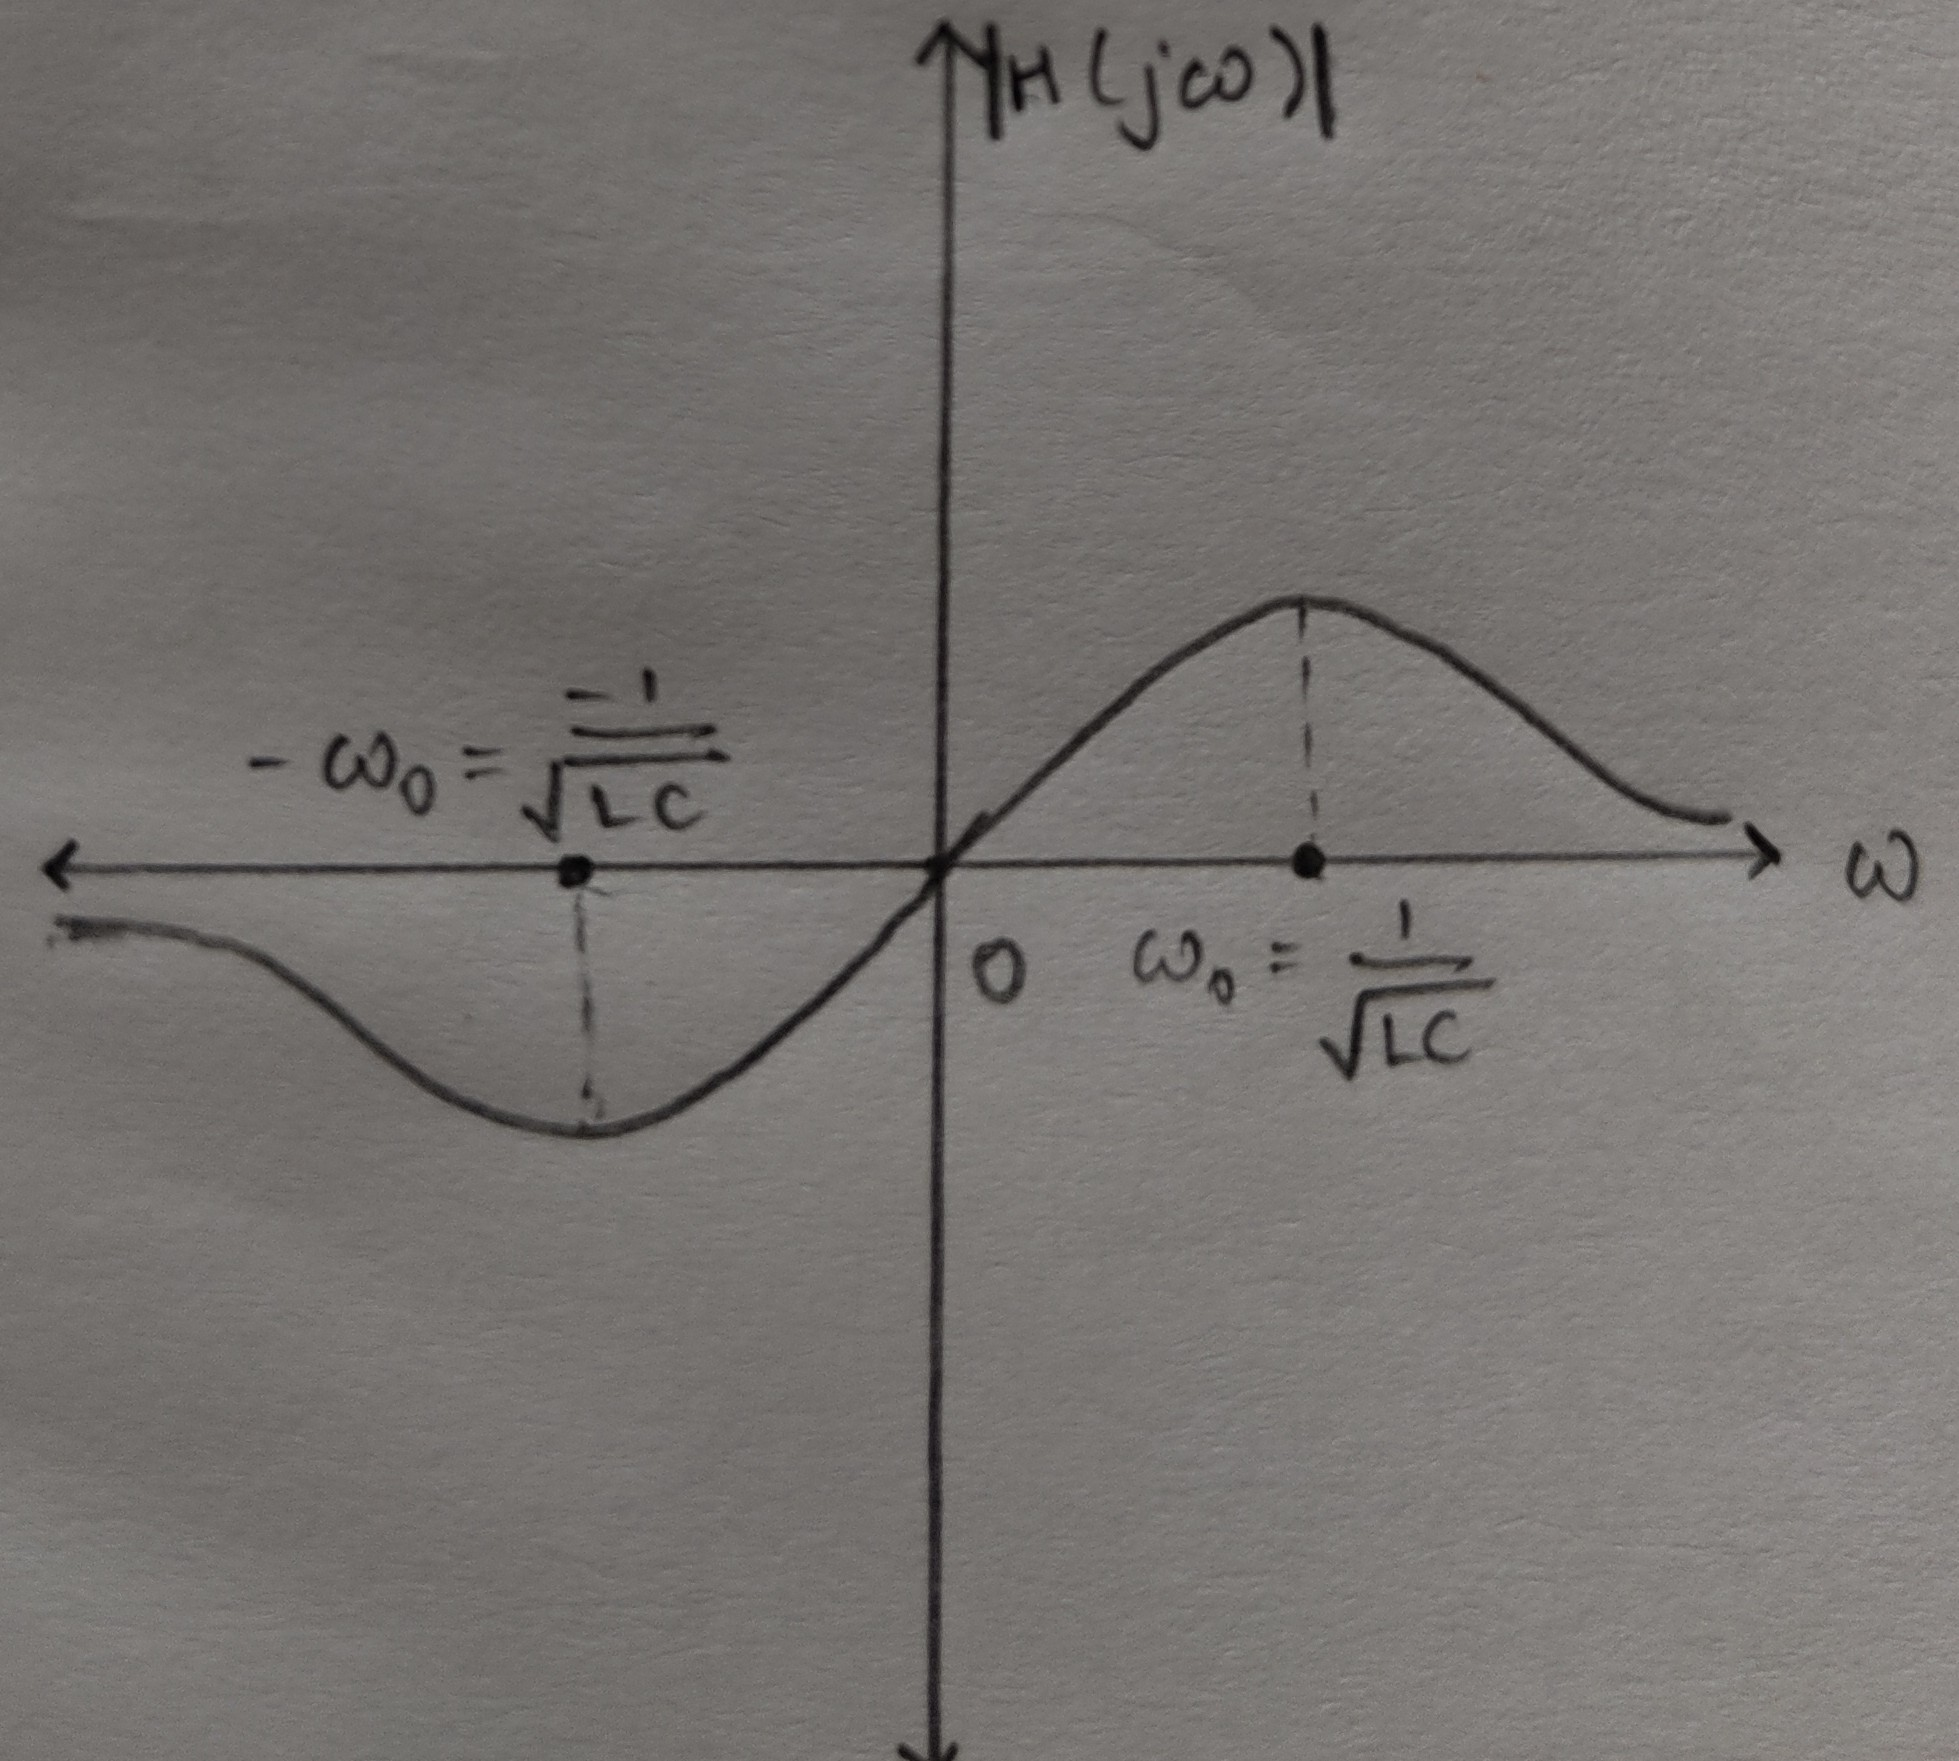
\includegraphics[width=\columnwidth]{figs/mag-resp.jpg}
        \caption{Graph of magnitude response \(\abs{H\brak{j\omega}}\).}
        \label{fig:mag-resp}
    \end{figure}

    \item We rewrite \eqref{eq:imp-resp-mag} as
    \begin{equation}
        \abs{H\brak{j\omega}} = \frac{\frac{R}{L}}{\sqrt{\brak{\frac{1}{LC\omega}-\omega}^2 + \brak{\frac{R}{L}}^2}}.
    \end{equation}
    Clearly, the maximum in \eqref{eq:imp-resp-mag} is maximized on minimizing
    the denominator, thus we must have
    \begin{align}
        \frac{1}{LC\omega} - \omega &= 0 \\
        \implies \omega = \frac{1}{\sqrt{LC}} &= \omega_0.
        \label{eq:reso-freq}
    \end{align}
    Thus, we obtain
    \begin{equation}
        H_{max} \define \abs{H\brak{j\omega_0}} = 1.
        \label{eq:h-max}
    \end{equation}
    This means that at resonance, the entire input voltage appears across the
    resistor.

    \item We have to solve for \(\omega_c\), where
    \begin{equation}
        \abs{H\brak{j\omega_c}} = \frac{1}{\sqrt{2}}H_{max} = \frac{1}{\sqrt{2}}.
        \label{eq:h-wc}
    \end{equation}
    Using \eqref{eq:imp-resp-mag} and squaring on both sides,
    \begin{align}
        &\frac{\brak{\frac{R}{L}\omega_c}^2}{\brak{\frac{1}{LC}-\omega_c^2}^2 + \brak{\frac{R}{L}\omega_c}^2} = \frac{1}{2} \\
        &\brak{\frac{R}{L}\omega_c}^2 = \brak{\frac{1}{LC} - \omega_c^2}^2 \\
        &\omega_c^2 \pm \frac{R}{L}\omega_c - \frac{1}{LC} = 0 \\
        &\omega_c = \pm \frac{R}{2L} \pm \sqrt{\frac{R^2}{4L^2} + \frac{1}{4LC}}.
    \end{align}
    Forcing \(\omega_c\) to be positive, we get the 3dB-cutoff frequencies to be
    \begin{equation}
        \omega_{c2}, \omega_{c1} = \sqrt{\frac{R^2}{4L^2} + \frac{1}{4LC}} \pm \frac{R}{2L}.
        \label{eq:omega-cutoff}
    \end{equation}
    Therefore, the 3-dB bandwidth parameter,
    \begin{equation}
        \beta = \omega_{c2} - \omega_{c1} = \frac{R}{L}.
        \label{eq:3db-bandwidth}
    \end{equation}
    Hence, the Q-factor is
    \begin{equation}
        Q = \frac{\omega_0}{\beta} = \frac{1}{R}\sqrt{\frac{L}{C}}.
        \label{eq:q-factor}
    \end{equation}

    \item Define
    \begin{equation}
        \Omega_0 \define 2\pi{}f_0.
        \label{eq:Omega-def}
    \end{equation}
    The Laplace transform of the input waveform is
    \begin{equation}
        X\brak{s} = \frac{s\cos\theta-\Omega_0\sin\theta}{s^2 + \Omega_0^2}.
        \label{eq:X-s-9}
    \end{equation}
    We have three cases.
    \begin{enumerate}
        \item \(\alpha < \omega_0\). Using \eqref{eq:H-s-underdamping},
        \begin{align}
            Y\brak{s} &= \frac{2\alpha{}s\brak{s\cos\theta - \Omega_0\sin\theta}}{\brak{\brak{s+\alpha}^2+\omega^2}\brak{s^2+\Omega_0^2}} \\
            &= \frac{P_1}{s+\alpha-j\omega} + \frac{P_2}{s+\alpha+j\omega} \nonumber \\
            &+ \frac{P_3}{s-j\Omega_0} + \frac{P_4}{s+j\Omega_0},
            \label{eq:part-frac-underdamping}
        \end{align}
        where we have to solve for \(P_i,\ i \in \cbrak{1,2,3,4}\). From 
        \eqref{eq:part-frac-underdamping}, we see that
        \begin{align}
            &P_1\brak{s+\alpha+j\omega}\brak{s^2+\Omega_0^2} \nonumber \\
            &+ P_2\brak{s+\alpha-j\omega}\brak{s^2+\Omega_0^2} \nonumber \\
            &+ P_3\brak{s+j\Omega_0}\brak{\brak{s+\alpha}^2+\omega^2} \nonumber \\
            &+ P_4\brak{s-j\Omega_0}\brak{\brak{s+\alpha}^2+\omega^2} \nonumber \\
            &= 2\alpha{}s\brak{s\cos\theta-\Omega_0\sin\theta}
            \label{eq:part-eq-underdamping}
        \end{align}
        Setting \(s = -\alpha+j\omega\) in \eqref{eq:part-eq-underdamping},
        \begin{equation}
            P_1 = \frac{\alpha\brak{\alpha-j\omega}\brak{\brak{\alpha-j\omega}\cos\theta+\Omega_0\sin\theta}}{j\omega\brak{\brak{\alpha-j\omega}^2+\Omega_0^2}}.
            \label{eq:P-1-def-underdamping}
        \end{equation}
        Setting \(s = -\alpha-j\omega\) in \eqref{eq:part-eq-underdamping},
        \begin{align}
            P_2 &= \bar{P_1} \\
                &= \frac{j\alpha\brak{\alpha+j\omega}\brak{\brak{\alpha+j\omega}\cos\theta+\Omega_0\sin\theta}}{\omega\brak{\brak{\alpha+j\omega}^2+\Omega_0^2}}.
            \label{eq:P-2-def-underdamping}
        \end{align}
        Setting \(s = j\Omega_0\) in \eqref{eq:part-eq-underdamping},
        \begin{equation}
            P_3 = \frac{j\alpha\Omega_0e^{j\theta}}{\brak{\alpha+j\Omega_0}^2+\omega^2}
            \label{eq:P-3-def-underdamping}
        \end{equation}
        Setting \(s = -j\Omega_0\) in \eqref{eq:part-eq-underdamping},
        \begin{align}
            P_4 &= \bar{P_3} \\
                &= \frac{\alpha\Omega_0e^{-j\theta}}{j\brak{\brak{\alpha-j\Omega_0}^2+\omega^2}}
            \label{eq:P-4-def-underdamping}
        \end{align}
        Thus, taking the inverse Laplace transform of
        \eqref{eq:part-frac-underdamping}, and using
        \eqref{eq:P-1-def-underdamping}, \eqref{eq:P-2-def-underdamping},
        \eqref{eq:P-3-def-underdamping}, \eqref{eq:P-4-def-underdamping},
        \begin{equation}
            y\brak{t} = 2\re\brak{P_1e^{-\brak{\alpha-j\omega}t}+P_3e^{j\Omega_0t}}u\brak{t}
            \label{eq:y-t-cos-underdamping}
        \end{equation}

        \item \(\alpha = \omega_0\). Using \eqref{eq:H-s-crit},
        \begin{align}
            Y\brak{s} &= \frac{2\alpha{}s\brak{s\cos\theta-\Omega_0\sin\theta}}{\brak{s+\alpha}^2\brak{s^2+\Omega_0^2}} \\
            &= \frac{P_1}{s+\alpha} + \frac{P_2}{\brak{s+\alpha}^2} \nonumber \\
            &+ \frac{P_3}{s-j\Omega_0} + \frac{P_4}{s+j\Omega_0},
            \label{eq:part-frac-crit}
        \end{align}
        where we have to solve for \(P_i,\ i \in \cbrak{1,2,3,4}\). From 
        \eqref{eq:part-frac-crit}, we see that
        \begin{align}
            &P_1\brak{s+\alpha}\brak{s^2+\Omega_0^2} + P_2\brak{s^2+\Omega_0^2} \nonumber \\
            &+ P_3\brak{s+\alpha}^2\brak{s+j\Omega_0} \nonumber \\
            &+ P_4\brak{s+\alpha}^2\brak{s-j\Omega_0} \nonumber \\
            &= 2\alpha{}s\brak{s\cos\theta-\Omega_0\sin\theta}
            \label{eq:part-eq-crit}
        \end{align}
        Setting \(s = -\alpha\) in \eqref{eq:part-eq-crit},
        \begin{equation}
            P_2 = \frac{2\alpha^2\brak{\alpha\cos\theta+\Omega_0\sin\theta}}{\alpha^2+\Omega_0^2}.
            \label{eq:P-2-def-crit}
        \end{equation}
        Setting \(s = j\Omega_0\) in \eqref{eq:part-eq-crit},
        \begin{equation}
            P_3 = \frac{j\alpha\Omega_0e^{j\theta}}{\brak{\alpha+j\Omega_0}^2}
            \label{eq:P-3-def-crit}
        \end{equation}
        Setting \(s = -j\Omega_0\) in \eqref{eq:part-eq-crit},
        \begin{align}
            P_4 &= \bar{P_3} \\
                &= \frac{\alpha\Omega_0e^{-j\theta}}{j\brak{\alpha-j\Omega_0}^2}.
            \label{eq:P-4-def-crit}
        \end{align}
        Equating the coefficient of \(s^3\) on both sides of \eqref{eq:part-eq-crit},
        \begin{align}
            P_1 &= -\brak{P_3 + P_4} \\
                &= \frac{2\alpha\Omega_0\brak{2\alpha\Omega_0\cos\theta-\brak{\alpha^2-\Omega_0^2}\sin\theta}}{\brak{\alpha^2+\Omega_0^2}^2}.
            \label{eq:P-1-def-crit}
        \end{align}
        Taking the inverse Laplace transform of \eqref{eq:part-frac-crit},
        and using \eqref{eq:P-1-def-crit}, \eqref{eq:P-2-def-crit},
        \eqref{eq:P-3-def-crit} and \eqref{eq:P-4-def-crit},
        \begin{equation}
            y\brak{t} = \brak{e^{-\alpha{}t}\brak{P_1 + P_2t} + 2\re\brak{P_3e^{j\Omega_0t}}}u\brak{t}.
            \label{eq:y-t-crit}
        \end{equation}

        \item \(\alpha > \omega_0\). Using \eqref{eq:H-s-overdamping},
        \begin{align}
            Y\brak{s} &= \frac{2\alpha{}s\brak{s\cos\theta-\Omega_0\sin\theta}}{\brak{\brak{s+\alpha}^2-\beta^2}\brak{s^2+\Omega_0^2}} \\
                      &= \frac{P_1}{s+\alpha-\beta} + \frac{P_2}{s+\alpha+\beta} \nonumber \\
                      &+ \frac{P_3}{s-j\Omega_0} + \frac{P_4}{s+j\Omega_0}.
                      \label{eq:part-frac-overdamping}
        \end{align}
        Using \eqref{eq:part-frac-overdamping},
        \begin{align}
            &P_1\brak{s+\alpha+\beta}\brak{s^2+\Omega_0^2} \nonumber \\
            &+ P_2\brak{s+\alpha-\beta}\brak{s^2+\Omega_0^2} \nonumber \\
            &+ P_3\brak{s+j\Omega_0}\brak{\brak{s+\alpha}^2-\beta^2} \nonumber \\
            &+ P_4\brak{s-j\Omega_0}\brak{\brak{s+\alpha}^2-\beta^2} \nonumber \\
            &= 2\alpha{}s\brak{s\cos\theta-\Omega_0\sin\theta}.
            \label{eq:part-eq-overdamping}
        \end{align}
        Setting \(s = -\alpha+\beta\) in \eqref{eq:part-eq-overdamping},
        \begin{equation}
            P_1 = \frac{\alpha\brak{\alpha-\beta}\brak{\brak{\alpha-\beta}\cos\theta+\Omega_0\sin\theta}}{\beta\brak{\brak{\alpha-\beta}^2+\Omega_0^2}}.
            \label{eq:P-1-def-overdamping}
        \end{equation}
        Setting \(s = -\alpha-\beta\) in \eqref{eq:part-eq-overdamping},
        \begin{equation}
            P_2 = \frac{\alpha\brak{\alpha+\beta}\brak{\brak{\alpha+\beta}\cos\theta+\Omega_0\sin\theta}}{\beta\brak{\brak{\alpha+\beta}^2+\Omega_0^2}}.
            \label{eq:P-2-def-overdamping}
        \end{equation}
        Setting \(s = j\Omega_0\) in \eqref{eq:part-eq-overdamping},
        \begin{equation}
            P_3 = \frac{j\alpha\Omega_0e^{j\theta}}{\brak{\alpha+j\Omega_0}^2-\beta^2}.
            \label{eq:P-3-def-overdamping}
        \end{equation}
        Setting \(s = -j\Omega_0\) in \eqref{eq:part-eq-overdamping},
        \begin{align}
            P_4 &= \bar{P_3} \\
                &= \frac{\alpha\Omega_0e^{-j\theta}}{j\brak{\brak{\alpha-j\Omega_0}^2-\beta^2}}.
            \label{eq:P-4-def-overdamping}
        \end{align}
        Taking the inverse Laplace transform of \eqref{eq:part-frac-overdamping},
        and using \eqref{eq:P-1-def-overdamping}, \eqref{eq:P-2-def-overdamping},
        \eqref{eq:P-3-def-overdamping} and \eqref{eq:P-4-def-overdamping},
        \begin{multline}
            y\brak{t} = \lbrak{e^{-\alpha{}t}\brak{P_1e^{\beta{}t} + P_2e^{-\beta{}t}}} \\
            \rbrak{+ 2\re\brak{P_3e^{j\Omega_0t}}}u\brak{t}.
            \label{eq:y-t-overdamping}
        \end{multline}
    \end{enumerate}

    \item The Laplace transform of the given input is
    \begin{equation}
        X\brak{s} = \frac{1}{s}.
        \label{eq:X-s-10}
    \end{equation}
    Applying \eqref{eq:X-s-10} in \eqref{eq:s-trans-func}, and using
    \eqref{eq:alpha-def}, \eqref{eq:omega-0-def},
    \begin{equation}
        Y\brak{s} = \frac{2\alpha}{\brak{s+\alpha}^2 + \brak{\omega_0^2-\alpha^2}}.
        \label{Y-s-10}
    \end{equation}
    Three cases arise.
    \begin{enumerate}
        \item \(\alpha < \omega_0\). Using \eqref{eq:omega-def} and
        \eqref{eq:H-s-underdamping},
        \begin{align}
            Y\brak{s} &= \frac{2\alpha}{\omega}\frac{\omega}{\brak{s+\alpha}^2+\omega^2} \\
            \implies y\brak{t} &= \mathcal{L}^{-1}\sbrak{Y\brak{s}} \nonumber \\
            &= \frac{2\alpha}{\omega}e^{-\alpha{}t}u\brak{t}\sin\omega{}t.
        \end{align}

        \item \(\alpha = \omega_0\). Using \eqref{eq:H-s-crit},
        \begin{align}
            Y\brak{s} &= \frac{2\alpha}{\brak{s+\alpha}^2} \\
            \implies y\brak{t} &= \mathcal{L}^{-1}\sbrak{Y\brak{s}} \nonumber \\
            &= 2\alpha{}e^{-\alpha{}t}u\brak{t}.
        \end{align}

        \item \(\alpha > \omega_0\). Using \eqref{eq:beta-def} and
        \eqref{eq:H-s-overdamping},
        \begin{align}
            Y\brak{s} &= \frac{2\alpha}{\beta}\frac{\beta}{\brak{s + \alpha}^2 - \beta^2} \\
            \implies y\brak{t} &= \mathcal{L}^{-1}\sbrak{Y\brak{s}} \nonumber \\
            &= \frac{2\alpha}{\beta}e^{-\alpha{}t}u\brak{t}\sinh\beta{}t.
        \end{align}
    \end{enumerate}
\end{enumerate}

\end{document}
